\section{Simulations}
\label{sec:simulations}
In this section we simulate the Ising model with various properties and examine
the properties of interest as functions of temperature $T$ and as functions of
lattice dimension $L$.
\subsection{$2\times2$ Ising with $T = 1$}
\label{sub:_2x2_ising_with_t_1_}
We assume we have a grid size of $2\times2$ as in
\cref{sub:a_2times2_ising_model}. We wish to consider these for a fixed
temperature $T' = 1.0$ in units of $Tk_B / J$.  We can therefore make the
following algebraic manipulations: Let $E'$ be the energy scaled by the
coupling constant $J$, that is $E' = E / J$. Similarly let $C_V' = C_V / k$ and
$\chi' = \chi J$. Let $N$ denote the number of Monte-Carlo cycles.

We can now easily compute the quantities using the closed form solutions given
in \cref{sub:a_2times2_ising_model}. The results are given in Table
\ref{tab:numerical comparison to analytical 2x2}. If we look at the error in
the numerical approximation, by means of the ratio between numerical and
analytical results we should expect a convergence towards 1. However, for the
specific heat, this is not the case, as the numerical results converge fairly
slowly. In \cref{fig:relative_error_1} we see that the magnetization and energy
converge quickly, after only two thousand cycles, the susceptibility follows
suit after some 10000 cycles while the specific heat never seem to converge,
even after a million cycles.
\begin{table}
  \centering
  \caption{Comparing numerical results to closed form analytical solutions for a $2\times2$ Ising model.}
  \label{tab:numerical comparison to analytical 2x2}
  \begin{tabular}{lcccc}
    \hline
    $N$ & $\langle E \rangle$ & $\langle \mathcal{M} \rangle$ & $C_V$ & $\chi$\\
    \hline
    100 & -2& 1 & 0& 0\\
    1000 & -2& 1& 0& 0 \\
    10000 & -1.9964& 0.67935& 0.0287482& 2.14783 \\
    100000 & -1.99654& 0.0276321& 0.0276321& 3.98085 \\
    1000000 & -1.99611& 0.05832& 0.0310754& 3.97991 \\
    \hline
    Analytical & -1.99598 & 0 & 0.03208 & 3.99330
  \end{tabular}
\end{table}
\begin{figure}
  \centering
  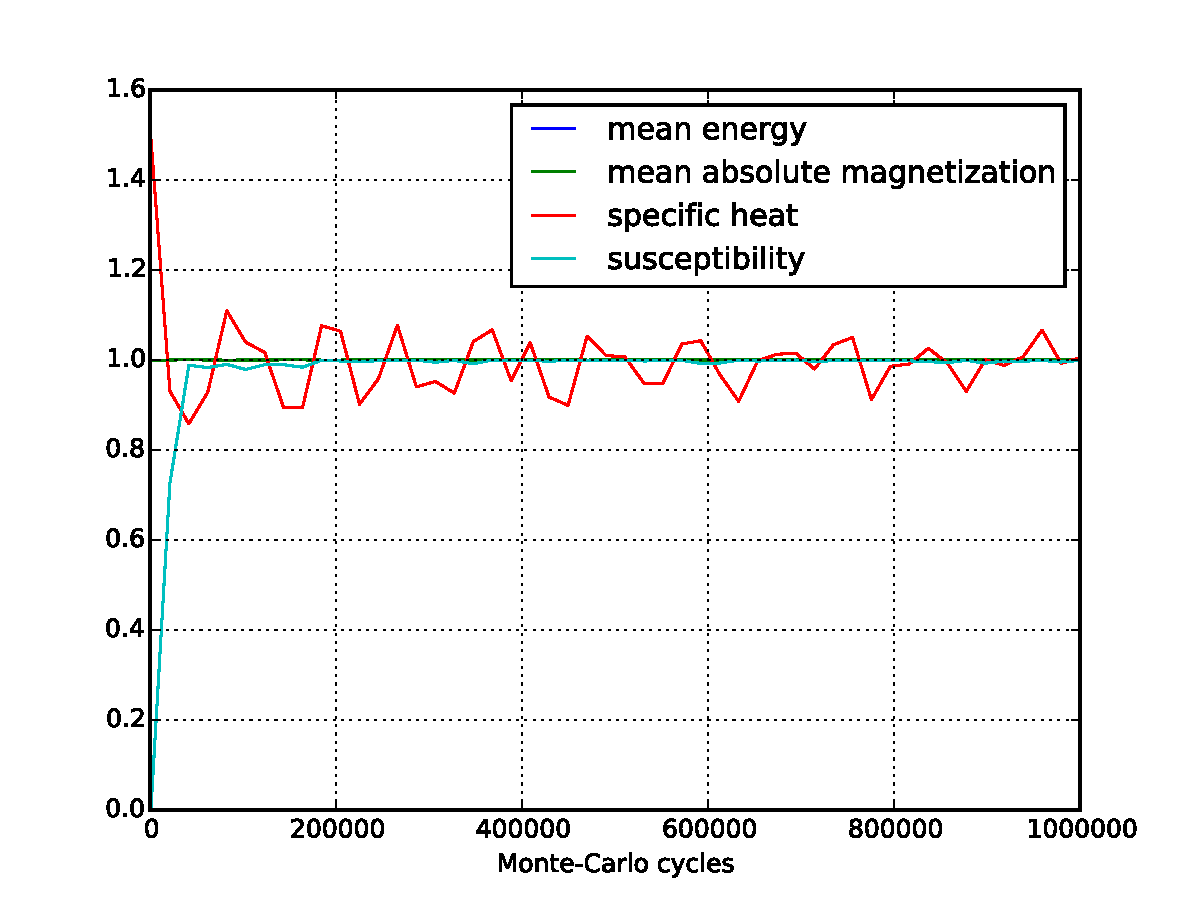
\includegraphics[width=0.8\linewidth]{task_b_million.pdf}
  \caption{This plot shows the convergence rate of the four quantities of
  interest. The magnetization and the energy converges after 2000 cycles, while
the susceptibility is slightly slower at 10000 cycles. The specific heat fails
to converge, even for a million cycles.}
  \label{fig:relative_error_1}
\end{figure}
\subsection{$20\times20$ Ising}
\label{sub:_20times20_ising}

We now consider a 20 by 20 lattice. We are interested in examining the number
of Monte-Carlo cycles needed to establish an equilibrium situation where it is
feasible to start calculating the expectation values. We start by plotting the
various expectation values as functions of the number of Monte-Carlo cycles.
We consider both an initial random configuration and an initial ordered
configuration for both the temperature $T = 1$ and $T = 2.4$.

While we're at it, we also keep track of the number of accepted configurations
and plot this as a function of temperature.
We see that for both random and ordered initial conditions, the system with a
temperature of $T = 1$ stabilizes fairly rapidly as can be seen in
\cref{fig:1_mc_ordered} and \cref{fig:1_mc_random} With a temperature of $T =
2.4$ however, the expectation values are a bit jittery at first, and seem to
somehow converge for upwards of 4000 cycles. This can be seen in
\cref{fig:2_mc_ordered} and \cref{fig:2_mc_random}.
\begin{figure}
  \centering
  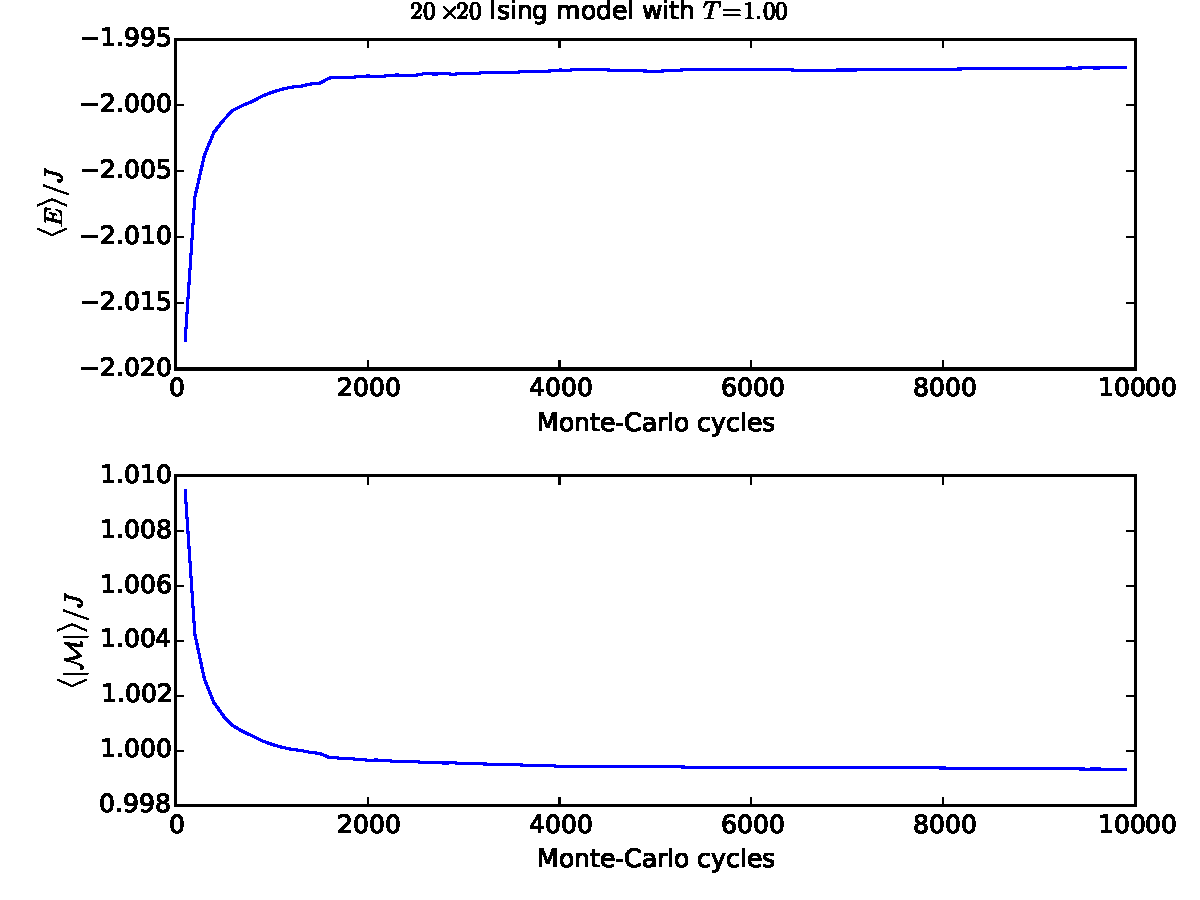
\includegraphics[width=0.8\linewidth]{1_mc_ordered.pdf}
  \caption{Plotting the expected energy and expected absolute magnetization as
  functions of the number of Monte-Carlo cycles. This system has a temperature
of $T = 1$ and an ordered initial configuration. In this situation the values
seem to stabilize around $2000$ cycles.}
  \label{fig:1_mc_ordered}
\end{figure}
\begin{figure}
  \centering
  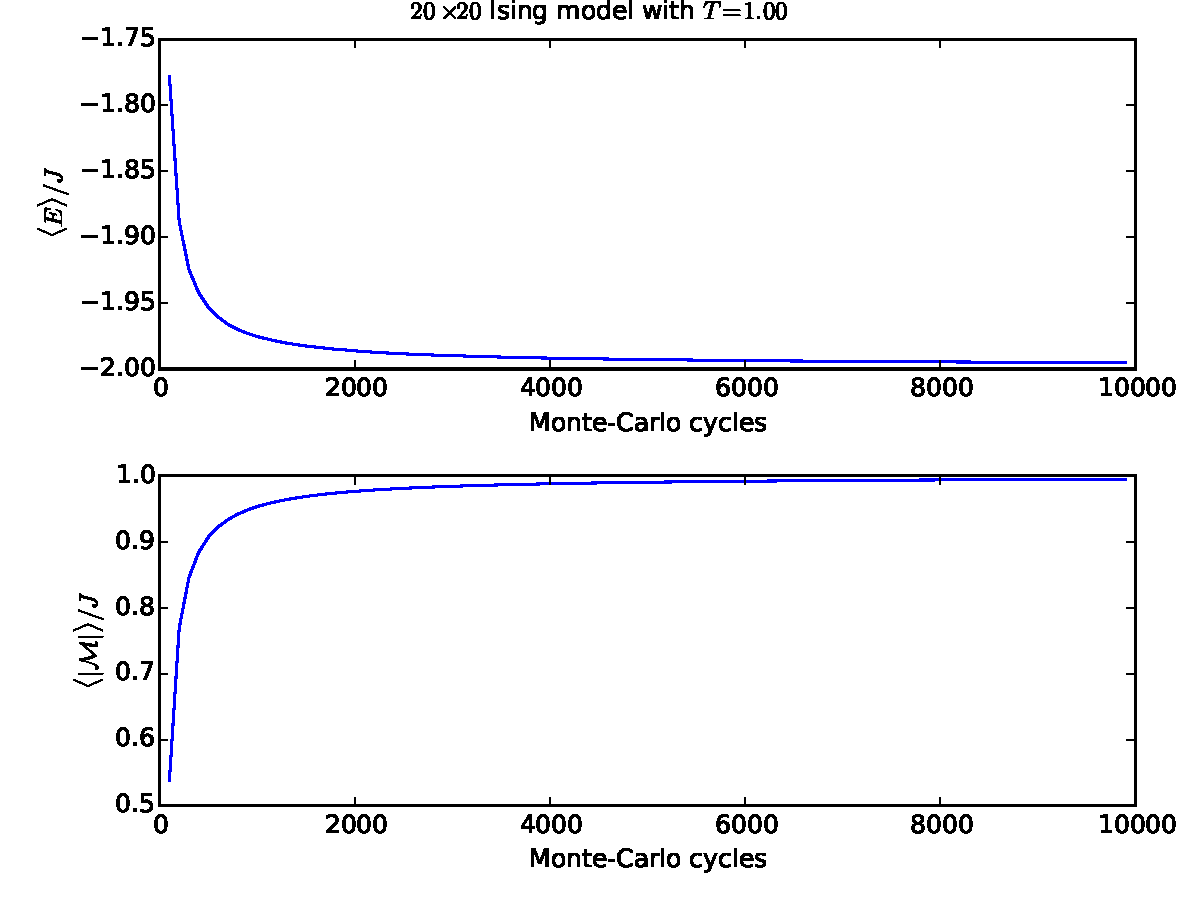
\includegraphics[width=0.8\linewidth]{1_mc_random.pdf}
  \caption{Plotting expected energy and expected absolute magnetization as
  functions of the numbers of the number of Monte-Carlo cycles. System has a
temperature of $T = 1$ with a random initial configuration. The system
stabilizes around $2000$ cycles.}
  \label{fig:1_mc_random}
\end{figure}

\begin{figure}
  \centering
  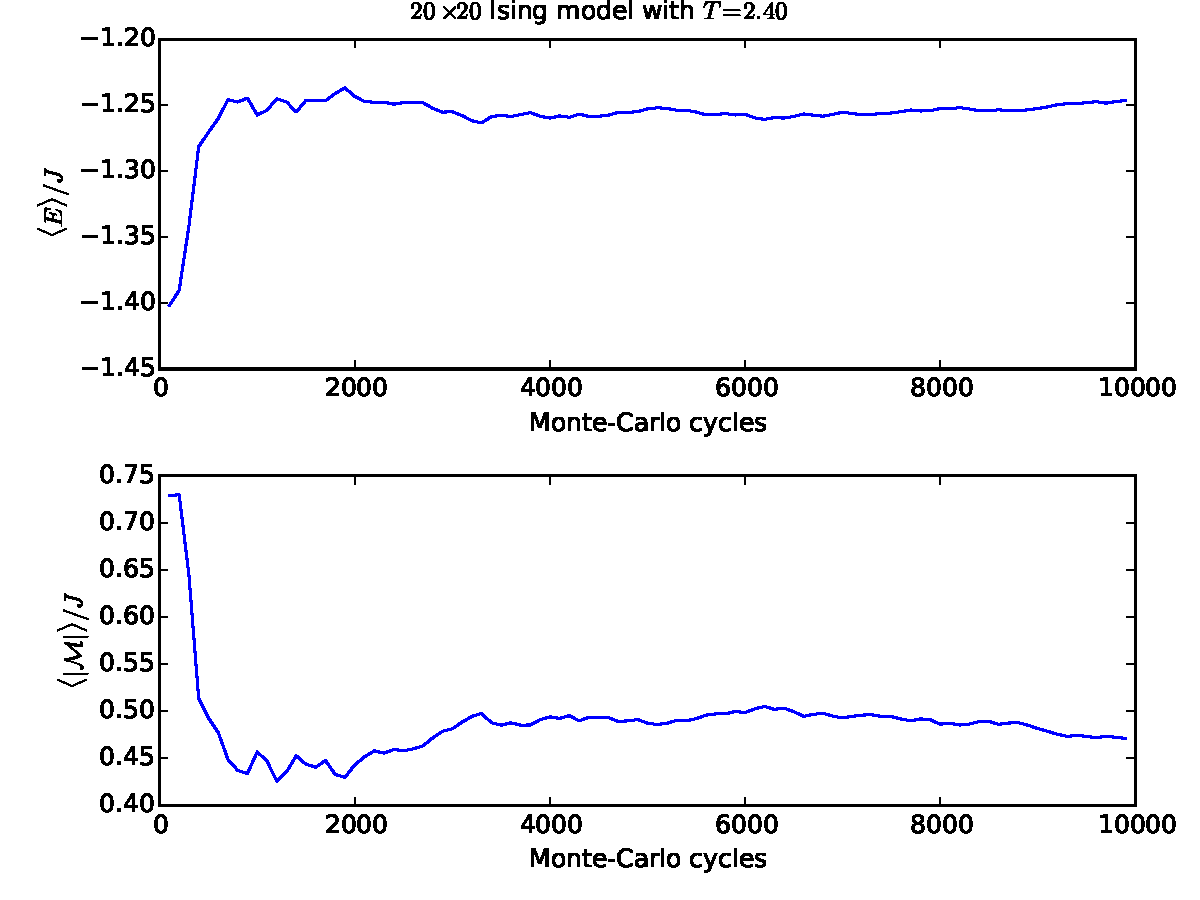
\includegraphics[width=0.8\linewidth]{2-4_mc_ordered.pdf}
  \caption{Plotting expected energy and expected absolute magnetization as
  functions of the numbers of the number of Monte-Carlo cycles. System has a
temperature of $T = 2.4$ with a random initial configuration. The system
stabilizes around $4000$ cycles.}
  \label{fig:2_mc_ordered}
\end{figure}

\begin{figure}
  \centering
  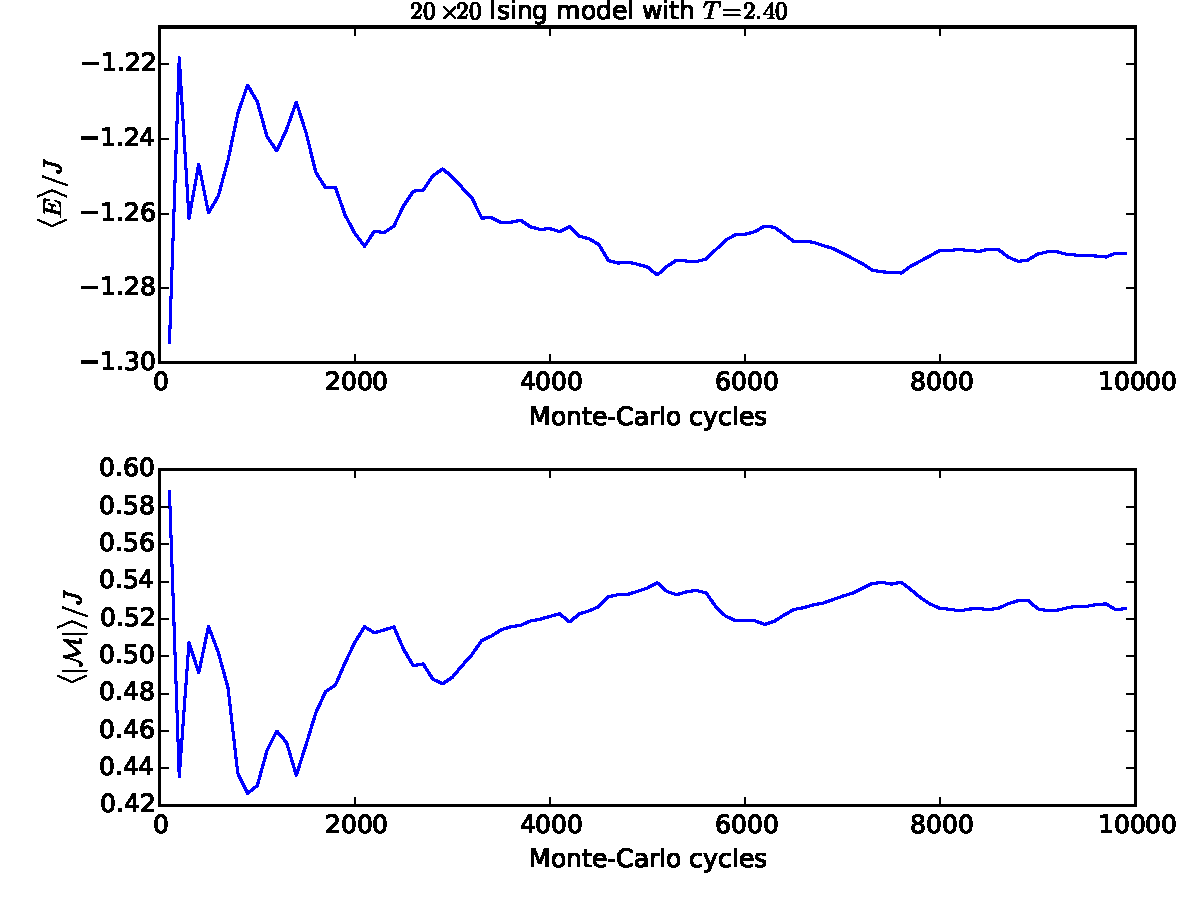
\includegraphics[width=0.8\linewidth]{2-4_mc_random.pdf}
  \caption{Plotting expected energy and expected absolute magnetization as
  functions of number of Monte-Carlo cycles. System has a temperature of $T =
2.4$ with a random initial configuration. The values seem to stabilize around
4000 cycles.}
  \label{fig:2_mc_random}
\end{figure}

When we consider the number of accepted states as a function of temperature, we
see that it increases drastically as the temperature increases. This is of
course in accordance with what we would assume if we were to just look at the
probability of any given state. As the temperature increases, the probability
of any arbitrary state becomes close to the probability of the most likely
state. You can view this as ''unlocking'' more possible states as the
temperature increases. The results are shown in \cref{fig:accepted_configs}.
\begin{figure}
  \centering
  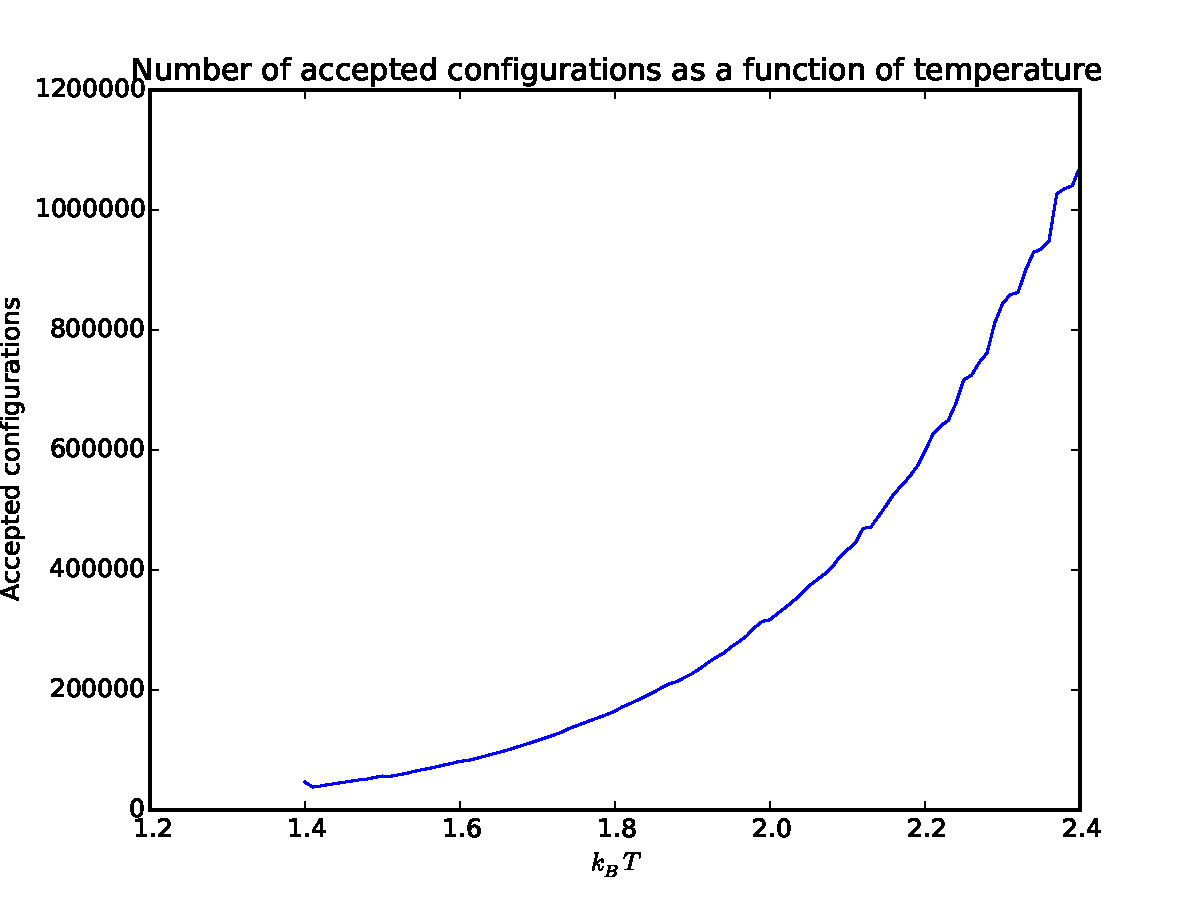
\includegraphics[width=0.8\linewidth]{accepted_configs.pdf}
  \caption{Number of accepted configurations as a function of temperature. The
  results are in accordance with the mathematical expression for the
probability of any given state. This number is probably more interesting when
divided by total number of configurations looked at. We then get a graph
converging to some number $t \in \left[ 0, 1 \right]$ which corresponds to the
probability of a configuration being accepted.}
  \label{fig:accepted_configs}
\end{figure}

We also want to look at the probability $P(E)$ for this same system for both
temperatures of $T=1$ and $T = 2.4$. These are given in \cref{fig:probability
1} and \cref{fig:probability 24}. If we compare these results to the computed
energy variance $\sigma_E^2$ which for $T = 1$ is evaluated to $\sigma_E^2
\approx 9.34 $ and for $T = 2.4$ is evaluated to $\sigma_E^2 \approx  3229$ we
see that the plots seem reasonable.\footnote{These are not per spin as the
other quantities discussed.}
For $T = 1$ the standard deviation $\sigma_E \approx 3.06$ and for $T = 2.4$ it
is $\sigma_E \approx 56.8$. The physical interpretation of this is that when
increasing the temperature we accept more possible states as previously
discussed. We therefore see more energy states appearing further from the most
likely state.
\begin{figure}
  \centering
  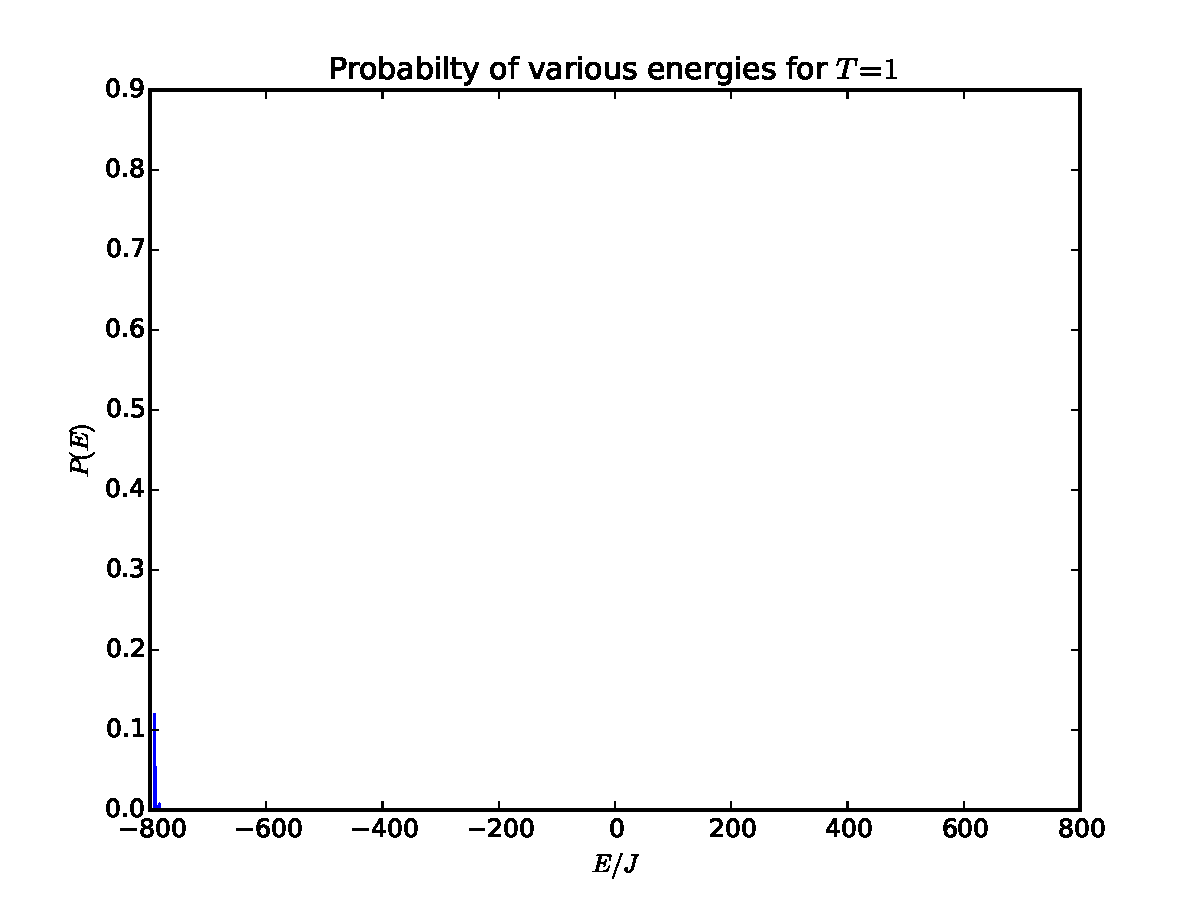
\includegraphics[width=0.8\linewidth]{probability_1.pdf}
  \caption{The probabilities of various energy levels in a Ising model with a
    temperature of $T = 1.0$. The energy states with a high probability are
    squashed all the way to the left which seems reasonable, since we start
    with an initially ordered configuration already in its ground state. Under
  low temperatures, the chance of escaping this ground state is very slim.}
  \label{fig:probability 1}
\end{figure}

\begin{figure}
  \centering
  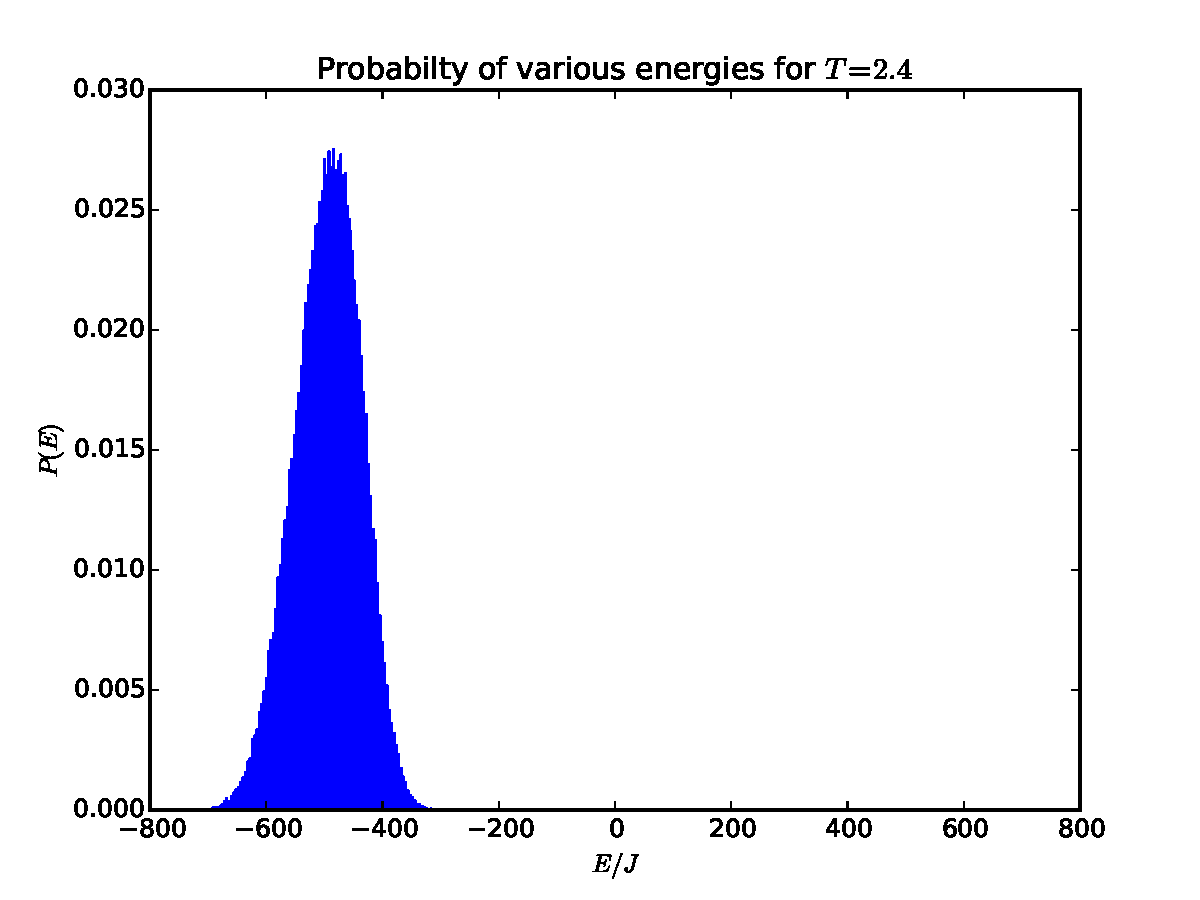
\includegraphics[width=0.8\linewidth]{probability_24.pdf}
  \caption{The probabilities of various energy levels in a Ising model with a
  temperature of $T = 2.4$. Here the energy states of interest are distributed
more evenly with the distribution centered at about $-500J$.}
  \label{fig:probability 24}
\end{figure}

\subsection{The critical temperature $T_C$ and the thermodynamical limit.}

In this section we examine the properties of the Ising model for various grid
sizes, and we fix our attention specifically to the temperature interval
$\left[ 2.0, 2.4 \right]$ as we know that the system undergoes a phase
transition for $T \approx 2.3$.

If we look at the plots given in \cref{fig:task_f_20}, \cref{fig:task_f_40},
\cref{fig:task_f_60} and \cref{fig:task_f_80} we see that increasing the grid
size changes the behavior of the system close to the critical temperature.
Firstly, we see that the susceptibility $\chi$ dramatically increase. As far as
I have understood, this means that near critical temperature, any change in
intensive parameters that does not depend on the number of particles in the
system constitutes a large change in magnetization. We also see that as the
absolute magnetization converges to zero for increasing grid size near critical
temperature which definitely indicates that the system is undergoing a phase
transition. I used python to visualize this phase transition for a
$200\times200$-model. A \texttt{GIF} can be found in the
\texttt{animations}-folder.

Near the critical temperature it turns out we can look at the behavior of certain physical quantities by means of a power law.
For $\beta = 1/8$, $\alpha = 0$ and $\gamma = 7/4$ we see that the mean magnetization, specific heat and susceptibility as functions of temperature $T$ closely follows the following relations:
\begin{align*}
  \langle \mathcal{M}(T) \rangle &\sim \left( T - T_C \right)^\beta \\
  C_V(T) &\sim \left| T_C - T \right|^\alpha \\
  \chi(T) &\sim \left|T_C - T\right|^\gamma
\end{align*}
We can also look at the relation between a quantity computed for a finite
lattice size and the corresponding quantity in the thermodynamical limit. We
now wish to see whether we can approximate the thermodynamical limit using our
simulations of finite grids. The critical temperature as a function of lattice
size satisfies the following relation:
\begin{equation}
  \notag
  T_C(L) - T_C(L = \infty) = aL^{-1/v},
\end{equation}
where for $v = 1$ the exact result for critical temperature is ${kT_C/J = 2 /
\ln(1+\sqrt{2})}$ which evaluates to approximately 2.269. Rearranging the equation gives us
\begin{equation}
  T_C(L = \infty) = T_C(L) - aL^{-1/v}.
\end{equation}

We can now look at our simulations and see if we can approximate the critical
temperature in the thermodynamical limit. My simulations are not sufficiently
good for me to be able to point out the differences in critical temperature for
the various grid sizes, so all I know is that it is located between $T=2.25$
and $T=2.30$. That being said, the only reasonable assumption based on the
results my simulations produced is that $T_C$ is 2.275 for all lattice sizes.
However, this renders us unable to calculate the factor $a$ in the following relations:
\begin{align*}
  T_C(L = \infty) &= T_C(20) - a20^{-1} = 2.275 - \frac{a}{20}\\
  T_C(L = \infty) &= T_C(40) - a40^{-1} = 2.275 - \frac{a}{40}\\
  T_C(L = \infty) &= T_C(60) - a60^{-1} = 2.275 - \frac{a}{60}\\
  T_C(L = \infty) &= T_C(80) - a80^{-1} = 2.275 - \frac{a}{80}
\end{align*}
\begin{figure}
  \centering
  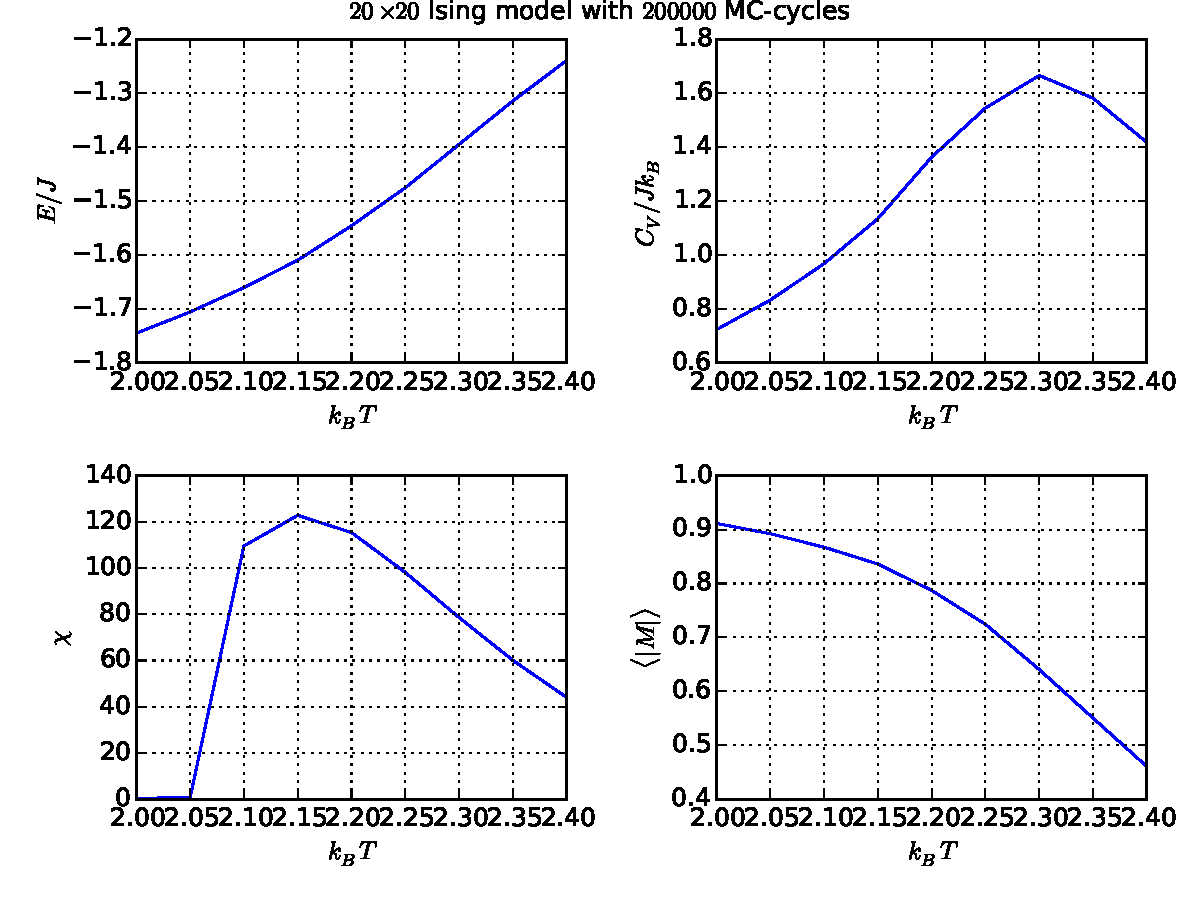
\includegraphics[width=0.8\linewidth]{task_f_20.pdf}
  \caption{Physical quantities near the critical temperature $T_C$ for a grid size of 20.}
  \label{fig:task_f_20}
\end{figure}

\begin{figure}
  \centering
  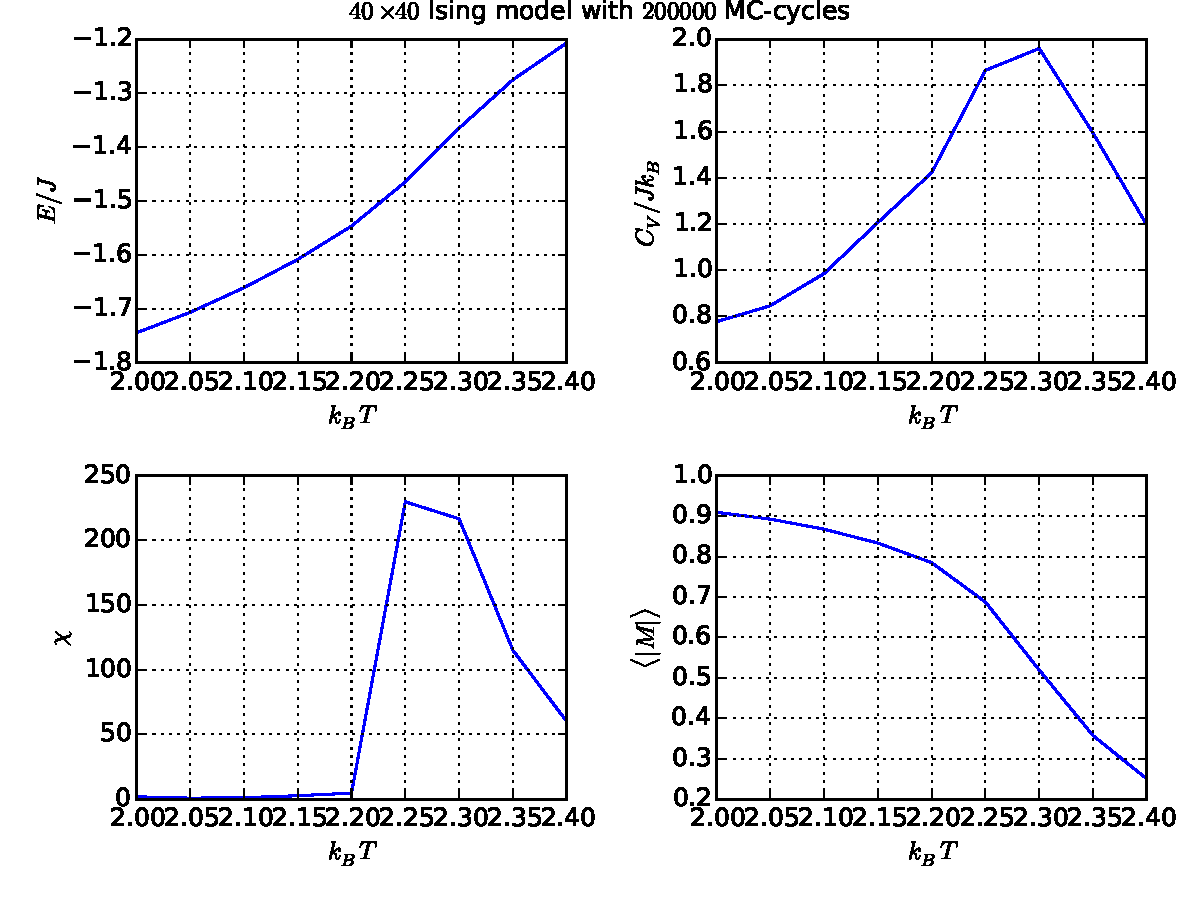
\includegraphics[width=0.8\linewidth]{task_f_40.pdf}
  \caption{Physical quantities near the critical temperature $T_C$ for a grid size of 40.}
  \label{fig:task_f_40}
\end{figure}

\begin{figure}
  \centering
  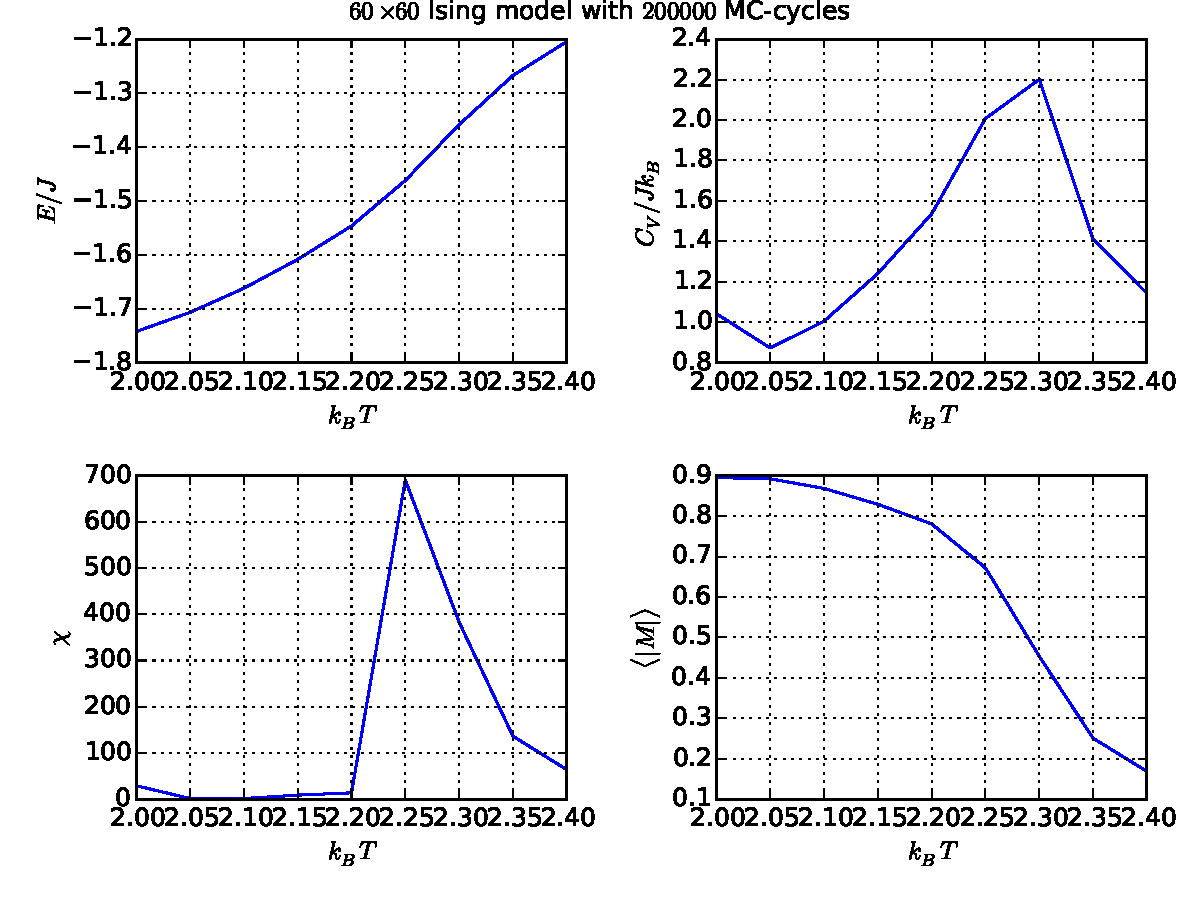
\includegraphics[width=0.8\linewidth]{task_f_60.pdf}
  \caption{Physical quantities near the critical temperature $T_C$ for a grid size of 60.}
  \label{fig:task_f_60}
\end{figure}

\begin{figure}
  \centering
  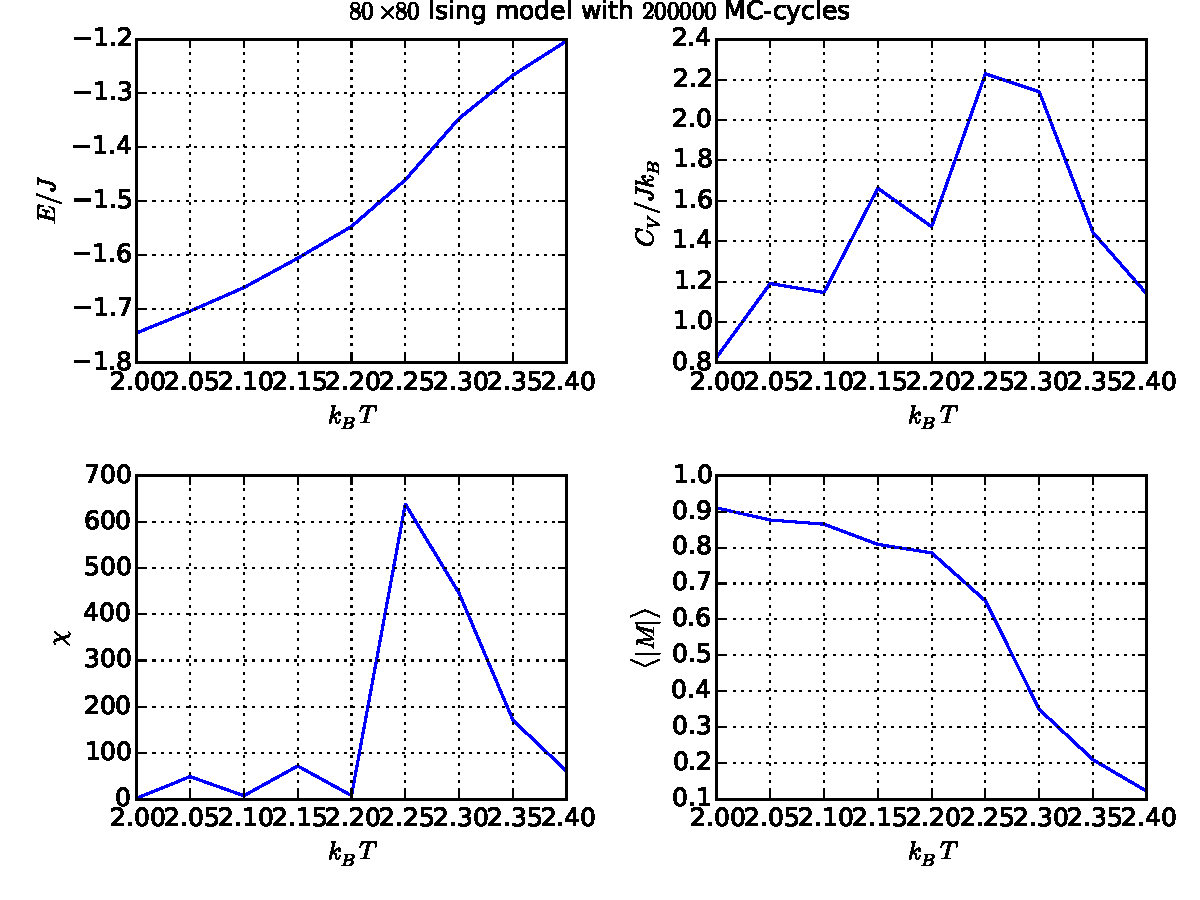
\includegraphics[width=0.8\linewidth]{task_f_80.pdf}
  \caption{Physical quantities near the critical temperature $T_C$ for a grid size of 80.}
  \label{fig:task_f_80}
\end{figure}
